\documentclass[border=0pt]{standalone} 
\usepackage[utf8]{inputenc}
\usepackage[T1]{fontenc}
% \usepackage[a4paper,vmargin=3cm]{geometry}
\usepackage{tikz}
\usetikzlibrary{arrows.meta}

% Third color palette - HHU color palette
% Primary colors
\definecolor{hhu-blau}{RGB}{0, 106, 179}        % hex: 006ab3 | RGB: 0, 106, 179
\definecolor{hhu-schwarz}{RGB}{0, 0, 0}        % hex: 000000 | RGB: 0, 0, 0

% Secondary colors
\definecolor{hhu-gruen}{RGB}{140, 177, 16}        % hex: 8cb110 | RGB: 140, 177, 16
\definecolor{hhu-orange}{RGB}{238, 127, 0}        % hex: ee7f00 | RGB: 238, 127, 0
\definecolor{hhu-rot}{RGB}{190, 10, 38}        % hex: be0a26 | RGB: 190, 10, 38
\definecolor{hhu-tuerkis}{RGB}{87, 186, 177}        % hex: 57bab1 | RGB: 87, 186, 177
\definecolor{hhu-dunkelblau}{RGB}{0, 57, 100}        % hex: 003964 | RGB: 0, 57, 100
\definecolor{hhu-eisblau}{RGB}{181, 203, 214}        % hex: b5cbd6 | RGB: 181, 203, 214


% Define color palette for arguments
\colorlet{nodeBaseOne}{hhu-blau!75}      
\colorlet{nodeBaseTwo}{hhu-tuerkis!75}
\colorlet{nodeBaseThree}{hhu-orange!50}
\colorlet{thesisBorder}{nodeBaseThree}


% Define colors for argument relations
\definecolor{supportColor}{RGB}{50,144,24}
\definecolor{attackColor}{RGB}{219,6,10}

\tikzset{
  % Styles for argument graph
  thesis/.style={rectangle,rounded corners, draw=thesisBorder, fill=white, thick, inner sep=3pt,text centered},
%   thesis/.style={rectangle,rounded corners, draw=thesisBorder, top color=white, bottom color=black!10, thick, inner sep=3pt,text centered},
  argument/.style={rectangle,rounded corners,draw=black, fill=nodeBaseThree, thick, inner sep=3pt,text centered},
  support/.style={->, >={Latex}, shorten >=1pt, thick,color=supportColor},
  attack/.style={->, >={Latex}, shorten >=1pt, thick,color=attackColor},
}


\begin{document}
  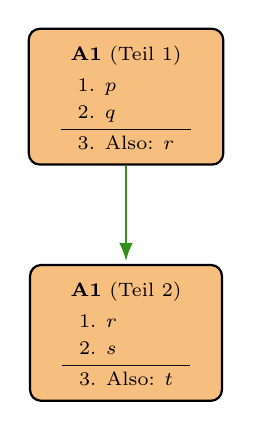
\begin{tikzpicture}
    \node[argument] (A1) at (2.0,-.5){
      \begin{tabular}{c}
        \scriptsize{\textbf{A1} (Teil 1)}\\[0.5ex]
        \scriptsize{
          \begin{tabular}{l}
              1. $p$\\[0.5ex]
              2. $q$ \\[0.5ex]
              \hline
              \noalign{\vskip 0.5ex}
              3. Also: $r$
          \end{tabular}
        }
      \end{tabular}
    };
    \node[argument] (A2) at (2,-3.5){
      \begin{tabular}{c}
        \scriptsize{\textbf{A1} (Teil 2)}\\[0.5ex]
        \scriptsize{
          \begin{tabular}{l}
              1. $r$\\[0.5ex]
              2. $s$ \\[0.5ex]
              \hline
              \noalign{\vskip 0.5ex}
              3. Also: $t$
          \end{tabular}
        }
      \end{tabular}
    };
    \draw[support] (A1) -- (A2); 
  \end{tikzpicture}%
\end{document}
